\begin{mysection}{Binary Search Trees}

\subsection{What is a BST?}
A \concept{binary search tree} is a data structure organized in a binary tree in which every node is an object containing a key (plus some satellite data), and some pointers \textit{left}, \textit{right}, \textit{p} which point to its left child, right child and parent nodes. If a child or parent is missing, the appropriate pointer attribute contains the value \NIL (so the root is the only node with parent \NIL). 


The keys in a BST are always stored in such a way as to satisfy the \textbf{BST invariant}:
\textit{``Let $x$ be a node in a BST. If $y$ is a node in the left subtree of x, then $y.key \leq x.key$. If $y$ is in the right subtree, then $y.key \geq x.key$.''}

\vspace*{1mm}
\begin{center}
    \tikzstyle{bstnode}=[circle, 
                         draw, 
                         fill=black!10,
                         inner sep=0pt,
                         text width=5mm,
                         align=center]
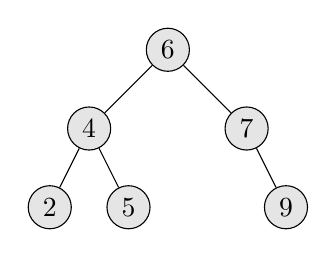
\begin{tikzpicture}
    \node [bstnode]{6} [level distance=10mm,sibling distance=20mm]
        child { node [bstnode]{4} [level distance=10mm ,sibling distance=10mm]
        child {node [bstnode] {2}}
        child {node [bstnode] {5}}
        }
        child {node [bstnode] {7} [level distance=10mm ,sibling distance=10mm]
        child[missing]{}
        child {node [bstnode] {9}}}
        ;
\end{tikzpicture}
\end{center}

The BST property allows us to visit all the keys in a binary search tree in sorted order by a simple recursive algorithm \procedure{Inorder-Tree-Walk}.

\begin{pseudocode}{Inorder-Tree-Walk}{x}
    \IF {$x \neq \NIL$}
        \STATE \procedure{Inorder-Tree-Walk}$(x.left)$
        \STATE print $x.key$
        \STATE \procedure{Inorder-Tree-Walk}$(x.right)$
    \ENDIF
\end{pseudocode}

\vspace*{3mm}
The correctness of the algorithm follows by induction using the BST invariant. And it takes linear time to visit all the tree, proven in the following theorem.

\begin{theorem}
If $x$ is the root of an $n$-node subtree, then the call \procedure{Inorder-Tree-Walk}$(x)$ takes $\Theta(n)$ time.
\end{theorem}
\begin{proof}
Let $T(n)$ be the running time of \procedure{Inorder-Tree-Walk} when it is called on the root of an $n$-node subtree. Since \procedure{Inorder-Tree-Walk} visits all $n$ nodes of the subtree, we have that $T(n) = \Omega(n)$. It remains to prove that $T(n) = O(n)$. \\

For an empty subtree, we have $T(0) = c$, for some constant $c > 0$. For $n > 0$, suppose \procedure{Inoder-Tree-Walk} is called ona node $x$  whose left subtree has $k$ nodes and whose right subtree has $n - k - 1$ nodes. Then the runnig time is bounded by $T(n) \leq T(k) + T(n - k - 1) + d$, for some constant $d > 0$ (reflecting upper bound time to execute body of \procedure{Inorder-Tree-Walk} excluding recursive calls). By the substitution method we show that $T(n) = O(n)$ by proving that $T(n) \leq (c+ d)n + c$. \\

For $n = 0$, $T(0) = c = (c + d) \cdot 0 + c$. And for $n > 0$ we have, 
\vspace*{-1mm}
\begin{align*}
    T(n) &\leq T(k) + T(n - k - 1) + d \\
         &= ((c + d)k + c) + ((c + d)(n - k - 1) + c) + d \\
         &= (c + d)n + c,
\end{align*}
which completes the proof.
\end{proof}


\subsection{Querying a BST}
We will present how the BST supports query operations in $O(h)$ time, where $h$ is the heigth of the tree (the length of the longest path from the root to a leaf).

\paragraph{Searching} 
 We use the \procedure{Tree-Search}, that given a pointer to the root of the tree and a key $k$, returns a pointer to a node with key $k$ if such exists; otherwise returns \NIL.

\begin{pseudocode}{Tree-Search}{x, k}
    \IF {$x == \NIL$ \OR $k == x.key$}
        \RETURN x
    \ELSIF {$k < x.key$}
        \RETURN \procedure{Tree-Search}$(x.left, k)$
    \ELSE 
        \RETURN \procedure{Tree-Search}$(x.right, k)$
    \ENDIF
\end{pseudocode}

\vspace{3mm}
The nodes encountered during the recursion form a simple path downward from te root of the tree, and thus the running time of \procedure{Tree-Search} is $O(h)$. We can rewrite the procedure in an iterative fashion by unrolling the recursion into a \textbf{while} loop, which is more efficient in most computers.

\begin{pseudocode}{Iterative-Tree-Search}{x, k}
    \WHILE {$x \neq \NIL$ \AND $k \neq x.key$}
        \IF {$k < x.key$}
            \STATE $x = x.left$
        \ELSE 
            \STATE $x = x.right$
        \ENDIF
    \ENDWHILE
    \RETURN x
\end{pseudocode}


\paragraph{Minimum and maximum}
We can find the minimum element in a BST by following the $left$ child pointers from the root until hit a leaf. 

\begin{pseudocode}{Tree-Minimum}{x}
    \WHILE {$x.left \neq \NIL$}
        \STATE $x = x.left$
    \ENDWHILE
    \RETURN x
\end{pseudocode}

\vspace{3mm}
The BST invariant guarantees the correctnes of the algorithm. If a node has no left subtree, then since every key in the right subtree is $\geq x.key$, the minimum key i the subtree roted at $x$ is $x.key$. If $x$ has a left subtree, then since no key in the right subtree is smaller than $x.key$ and no key in the left is greater than $x.key$, then the minimum key in the subtree rooted at $x$ resides in the left subtree rooted at $x.left$.

The algorithm for the maximum is symmetric.


\begin{pseudocode}{Tree-Maximum}{x}
    \WHILE {$x.right \neq \NIL$}
        \STATE $x = x.right$
    \ENDWHILE
    \RETURN x
\end{pseudocode}

\vspace{4mm}
Both procedures run in $O(h)$ time, since they visit all node sin a path downward from the root to the leftmost (and rightmost) leafs.


\paragraph{Successor and predecessor}
The successor of a node $x$ is the node with the smallest key greater than $x.key$. Using the structure of BST's we cnan obtain the successor of a node without comparing keys. The following gives the successor of a node $x$ in a BST if such exists, or NIL otherwise ($x$ has largest key in tree).

\begin{pseudocode}{Tree-Successor}{x}
    \IF {$x.right \neq \NIL$}
        \RETURN \procedure{Tree-Minimum}$(x.right)$
    \ENDIF
    \STATE $y = x.p$
    \WHILE {$y \neq \NIL$ \AND $x == y.right$}
        \STATE $x = y$
        \STATE $y = y.p$
    \ENDWHILE
    \RETURN y
\end{pseudocode}

\vspace{3mm}
We break the code for \procedure{Tree-Successor} into two cases. If the right subtree of $x$ is nonempty, then the successor of is just the leftmost node in $x$'s right subtree (minimum of right subtree). 

On the other hand, when $x$'s right subtree is empty and $x$ has a successor $y$, then $y$ is the lowest ancestor of $x$ whose left child is also an ancestor of $x$ (Proven in Exercise 12.2-6). \newline

The procedure \procedure{Tree-Predecessor} is symmetric to \procedure{Tree-Successor}. Both run in $O(h)$ time, since we either follow a path up the tree, or a path down the tree to a leaf.


\subsection{Insertion and deletion}
These operations cause the dynamic set represented by a BST to change. We can handle insertion easily, but deletion takes more care.

\paragraph{Insertion}
To insert a new value $\nu$ into a binary search tree $T$, we use the procedure \procedure{Tree-Insert}, which takes a node $z$ with key $\nu$, and $z.left = z.right = z.p = \NIL$. It modifies $T$ and $z$ to insert $z$ into the appropriate position in the tree $T$.

\begin{pseudocode}{Tree-Insert}{T, z}
    \STATE $y = \NIL$ ~~~ \COMMENT{Parent of $x$}
    \STATE $x = T.root$
    \WHILE {$x \neq \NIL$}
        \STATE $y = x$
        \IF {$z.key < x.key$}
            \STATE $x = x.left$
        \ELSE
            \STATE $x = x.right$
        \ENDIF
    \ENDWHILE

    \STATE $z.p = y$
    \IF {$y == \NIL$}
        \STATE $T.root = z$ ~~~ \COMMENT{Tree $T$ was empty}
    \ELSIF {$z.key < y.key$}
        \STATE $y.left = z$
    \ELSE \STATE $y.right = z$
    \ENDIF
\end{pseudocode}

\vspace{3mm} 
The procedure traces a path down the tree to a leaf, to find the position of the node $x$ to insert. Thus, the procedure \procedure{Tree-Insert} runs in $O(h)$ time on a tree of height $h$.


\vspace*{1mm}
\begin{center}
    \tikzstyle{bstnode}=[circle, 
                         draw, 
                         thin,
                         fill=black!10,
                         inner sep=0pt,
                         text width=5mm,
                         align=center]

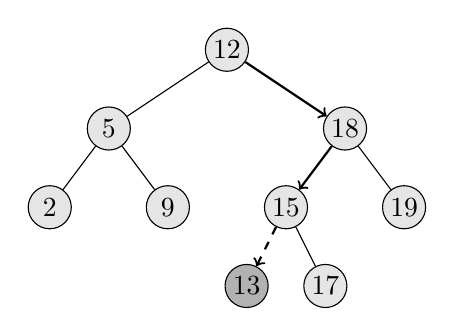
\begin{tikzpicture}
    % \node [bstindex] at (0,0.5) {1} [level distance=10mm ,sibling distance=30mm]
        % child {node [bstindex] {2} [level distance=10mm ,sibling distance=20mm] edge from parent [draw=white]
            % child {node [bstindex] {4} [level distance=10mm ,sibling distance=10mm] edge from parent [draw=white]
                % child {node [bstindex] {8} edge from parent [draw=white]}
                % child {node [bstindex] {9} edge from parent [draw=white]}}
            % child {node [bstindex] {5} [level distance=10mm ,sibling distance=10mm] edge from parent [draw=white]
                % child {node [bstindex] {10} edge from parent [draw=white]}
                % child [missing] { }}}
        % child {node [bstindex] {3} [level distance=10mm ,sibling distance=20mm] edge from parent [draw=white]
            % child {node [bstindex] {6} [level distance=10mm ,sibling distance=10mm] edge from parent [draw=white]}
            % child {node [bstindex] {7} [level distance=10mm ,sibling distance=10mm] edge from parent [draw=white]}};
    \node [bstnode] at (0,0) {12} [level distance=10mm,sibling distance=30mm]

        child {node [bstnode] {5} [level distance=10mm ,sibling distance=15mm]
            child {node [bstnode] {2} [level distance=10mm ,sibling distance=10mm]}
            child {node [bstnode] {9} [level distance=10mm ,sibling distance=10mm]}}
        child {node [bstnode] {18} [level distance=10mm ,sibling distance=15mm] edge from parent [->, thick]
            child {node [bstnode] {15} [level distance=10mm ,sibling distance=10mm]
                child {node [bstnode, fill=black!30] {13} edge from parent [dashed, thick]}
                child {node [bstnode] {17} edge from parent [-, thin]}}
            child {node [bstnode] {19} [level distance=10mm ,sibling distance=10mm] edge from parent [-, thin]}};
\end{tikzpicture}
\end{center}

As an example, we show the call to \procedure{Insert-Tree}$(13)$ to the above tree.



\end{mysection}
